\section{Aspect-Boost}
Aspect-Boost is an initial implementation of Aspect Programming on Artela, and it is a framework for any kind of blockchain to integrate to enable Aspect Programming on it. With Aspect-Boost, blockchain can support users to develop, deploy and execute Aspect on it. To integrate Aspect-Boost, blockchain nodes need to implement the adaptors of Aspect-Boots.

Aspect-Boots contains the following key components to boost the process of Aspect integration with different blockchains:

\begin{figure}[h]
  \centering
  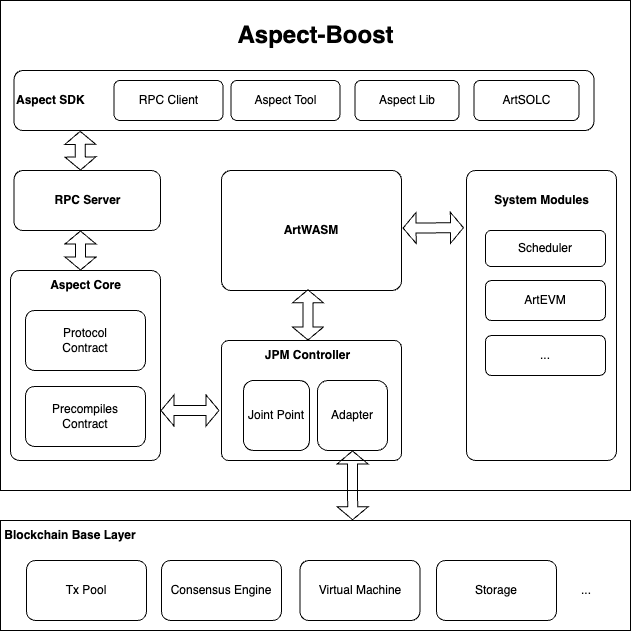
\includegraphics[width=0.4\textwidth]{sections/aspect-boost.png}
  \caption{Aspect-Boost Key Components}
\end{figure}

\begin{itemize}
  \item \textbf{Aspect Core.} The Aspect core is the management module within the Aspect framework and is primarily implemented through smart contracts. It mainly comprises protocol contracts and precompiled contracts. The Aspect core manages major lifecycle processes of Aspects, including deployment, upgrade, and binding, among others. This core module meticulously scrutinizes the ownership of the Aspect in relation to the operation initiator's address, maintains the binding relationships between Aspects and smart contracts, and handles the token settlement for Aspects.
  
  \item \textbf{JPM Controller.} The join point Model controller acts as a hub, connecting the blockchain base layer and the various components of the Aspect framework. It comes into action when specific transaction or block lifecycle stages are reached. Upon the activation of a join point, the JPM controller retrieves the relevant Aspects from the Aspect core, using the address of the smart contract that invoked the action. It then constructs an instance of the Aspect runtime (ArtWASM) to execute the Aspect. In addition, the JPM controller functions as a translator, mediating interactions between the base layer and the Aspect. When an Aspect is invoking base layer functions, the JPM controller's adaptor translates this system call into the corresponding request compatible with the blockchain platform, ensuring the successful execution of the call.
  
  \item \textbf{ArtWASM.} ArtWASM is a tailored WebAssembly (WASM) runtime specifically built for executing Aspects. Functioning as a sandbox, ArtWASM ensures the secure and efficient execution of Aspects within the blockchain environment. Its design incorporates significant optimizations, aligning it perfectly with the unique requirements of Aspect execution. ArtWASM serves as a bridge between Aspects, system modules, and the JPM controller by providing a comprehensive suite of runtime APIs. These APIs act as the conduit, enabling the necessary communication between these entities. When an Aspect initiates a system call, ArtWASM routes this call to the appropriate module, thereby facilitating seamless integration and interaction across the different components of the Aspect framework.
  
  \item \textbf{System Modules.} System modules comprise a set of system-level modules that can be seamlessly integrated with the blockchain base layer. These modules enhance the functionalities of dApps, enabling them to utilize the full potential of Aspects.
  
  \item \textbf{RPC Server.} The RPC server provides a set of interfaces that are compatible with existing blockchain platforms. These interfaces facilitate the processing of Aspect operations, ensuring interoperability between different platforms.
  
  \item \textbf{Aspect SDK.} The Aspect SDK equips developers with a set of tools to build rich dApps using Aspects. It simplifies the process of incorporating Aspects into dApps and allows for more advanced and flexible applications.
\end{itemize}

\subsection{ArtWASM}

ArtWASM is a secure and deterministic WASM Runtime implementation and it is designed for executing Aspect. It adheres to the design of the WASM Virtual Machine - a stack-based virtual machine constructed to execute WASM binary code.

\textbf{Gas metering.} Similar to a smart contract, gas metering has been implemented in ArtWASM to quantify resource usage by Aspect. This section will outline the implementation of gas metering in the WASM environment, drawing parallels with the gas metering models used in EVM and other blockchain execution environments.

We implemented gas metering in WASM via byte code instrumentation. This involves inserting additional instructions into the WASM code to monitor and control gas consumption.

Each WASM operation can be assigned a gas cost reflecting its complexity or the resources it uses. During the instrumentation process, additional WASM instructions are inserted before each operation to deduct the operation's gas cost from the total gas available. If the operation's gas cost exceeds the remaining gas, execution is halted, preventing excessive resource usage.

Consider a simple WASM function that adds two integers. In raw WASM, this might be represented by a sequence of instructions that load the integers from memory, perform the addition, and store the result back in memory.

To instrument this function with gas metering, additional instructions would be inserted before each operation. These instructions would deduct the gas cost of the operation from the total gas available. For example, if loading an integer from memory has a gas cost of 1, and performing an addition has a gas cost of 2, the instrumented WASM code would deduct these amounts from the total gas before performing the operations.

Instrumenting gas rules in WASM can bring a new level of resource management to the platform, drawing on principles similar to those used in Move and other blockchain platforms. While the specifics would need to be tailored to the WASM environment and the specific needs of its users, the underlying concept of gas as a means of metering resource usage is a powerful one that could greatly enhance the capabilities of the WASM platform.

\textbf{Gas rule for Aspect.} The gas model of eWASM is our main reference for ArtWASM. Endowed with an extensive selection of 64-bit Integer operations, data type alterations, and operations that are type-parametric, each operation incurs a unique gas expense to accurately mirror the computational exertion involved.

Every WASM opcode has a corresponding Intel IA-32 (x86) opcode (or a series of opcodes) assigned to it. These opcodes have a fixed cycle count, which Intel refers to as latency. This methodology uses a particular CPU model from the Sky Lake architecture (Intel Xeon Platinum 8175M, one of the most used CPUs by AWS EC2), similar to CPUs fabricated in 2018, to provide a reasonable average depiction of the Artela nodes. It is presumed that a 2.5 Ghz model embodies the average, with the clock rate approximately equaling 2,500,000,000 cycles per second. An additional supposition establishes that 1 second of CPU execution is equivalent to 10 million gas, meaning that 1 gas equals 0.1 us. This leads to 0.004 gas per cycle. Moreover, it is stipulated that the gas costs undergo regular adjustments, ideally every three years, in tandem with the consistent enhancements in CPUs and the routine upgrade of hardware for Artela nodes.

The WASM opcodes demand less computational power in contrast to EVM opcodes. EVM opcodes work on 256 bits of data, while WASM opcodes are restricted to a maximum of 64 bits. This means it takes four instructions, at the very least, to match EVM. Most arithmetic instructions in EVM cost 3 gas, translating to 0.75 gas for most 64-bit WASM instructions. This variance in processing requirements brings forth the notion of particles. Within the system, Aspect gas measurements are logged in a 64-bit variable with 4 decimal digits precision. When transitioning the WASM gas count to EVM gas, it is divided by 10,000 and rounded upwards. If the outcome is less than 0, it is then adjusted to 1.

\textbf{Runtime Pool.} During the lifecycle of a transaction or smart contract call, an instance of Aspect will be invoked multiple times. If the runtime instance is reinstantiated every time, it will bring significant delays to the execution. The following is some data we have measured:

\begin{center}
\begin{tabular}{|c|c|}
  \hline
  Method & Time Cost (micro-seconds) \\
  \hline
  NewEngine & 276 \\
  NewStore & 43 \\
  NewModule & 6395 \\
  NewLinker & 26 \\
  Function Link & 1034 \\
  \hline
\end{tabular}
\end{center}

ArtWASM's built-in runtime pool has made these overheads negligible by caching the runtime instances in an LRU cache and reusing the instances when needed.

\subsection{ArtEVM}

ArtEVM is an enhanced version of EVM provided in Aspect-Boost. ArtEVM is able to track all the state variable changes when a smart contract is executing, which provides an overview of account states for Aspect. In the meantime, ArtEVM can execute smart contract calls in parallel, maximizing the execution performance.

An improved version of the SOLC compiler has been implemented to actualize this feature. Additional state tracing opcode will be incorporated into the EVM bytecode using the pattern outlined below:

\begin{verbatim}
...
JOURNAL <-- Records the state before the SSTORE operation
SSTORE  <-- EVM Opcode that executes a change to the world state
JOURNAL <-- Records the state after the SSTORE operation
...
\end{verbatim}

By employing this pattern, the new instructions can systematically document state changes both preceding and following the SSTORE operation. With the help of the \texttt{journal} opcodes, the recorded state changes will save in the EVM context with the following format:

ArtEVM is capable of executing EVM smart contract calls in parallel. Traditionally, the execution of transactions in EVM is sequential due to potential data conflicts. However, ArtEVM leverages techniques including multi-version state-trie and block STM algorithm to analyze potential dependencies and conflicts between transactions, enabling them to be processed simultaneously without conflict. By grouping non-conflicting transactions together and processing them in parallel, ArtEVM can significantly increase the throughput and efficiency of smart contract execution. This parallel execution capability of ArtEVM enables it to handle a greater volume of transactions, thus boosting the scalability of the blockchain network.

ArtEVM is fully compatible with Ethereum's EVM. The state tracing feature can be toggled on or off by the compiler, providing developers with a choice: they can opt for a more cost-efficient smart contract or a more secure one.